\chapter*{Unused plots}
\label{App:Plots}
\begin{figure}[H]
    \centering
    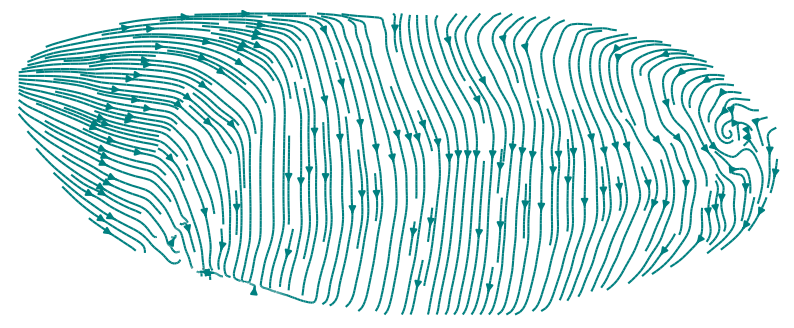
\includegraphics[width=1\linewidth]{chapters/Appendix/streamplot1.png}
\end{figure}
\begin{figure}[H]
    \centering
    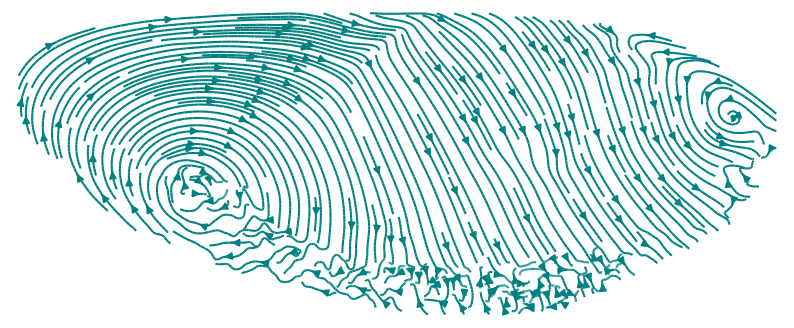
\includegraphics[width=1\linewidth]{chapters/Appendix/streamplot2.png}
    \caption{Seje stream plots}
    \label{fig:enter-label}
\end{figure}

\begin{figure}[H]
    \centering
    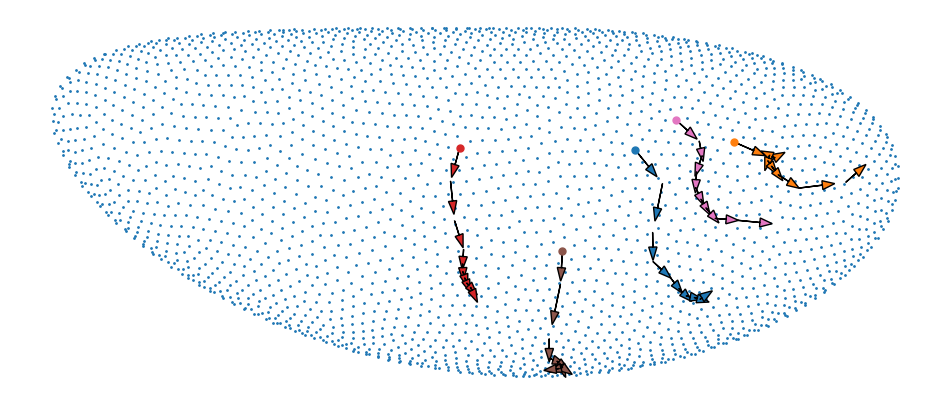
\includegraphics[width=1\linewidth]{chapters/Results/figures/movements.png}
    \caption{NOT TO SELF: Remove some of the cells -- it's cluttered!}
    \label{fig:GBMovements}
\end{figure}

\begin{figure}[H]
    \centering
    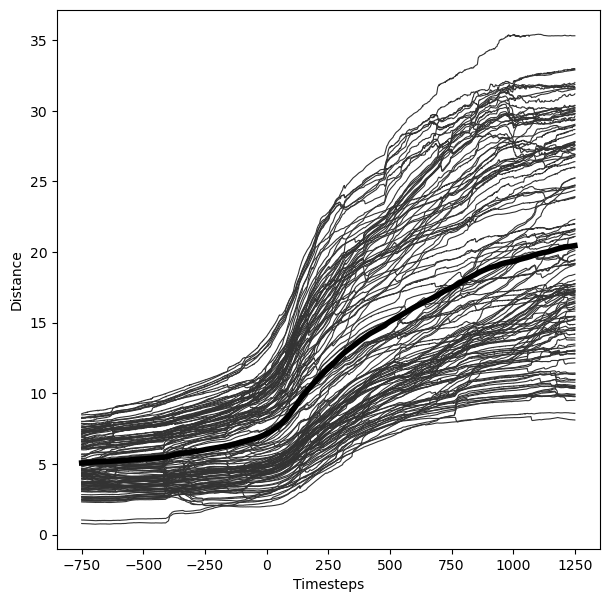
\includegraphics[width=1\linewidth]{chapters/Appendix/germbandMovementQuant.png}
    \caption{X-position of line of germ-band cells \url{https://www.ncbi.nlm.nih.gov/pmc/articles/PMC2801059/}}
    \label{fig:enter-label}
\end{figure}
\begin{figure}[H]
    \centering
    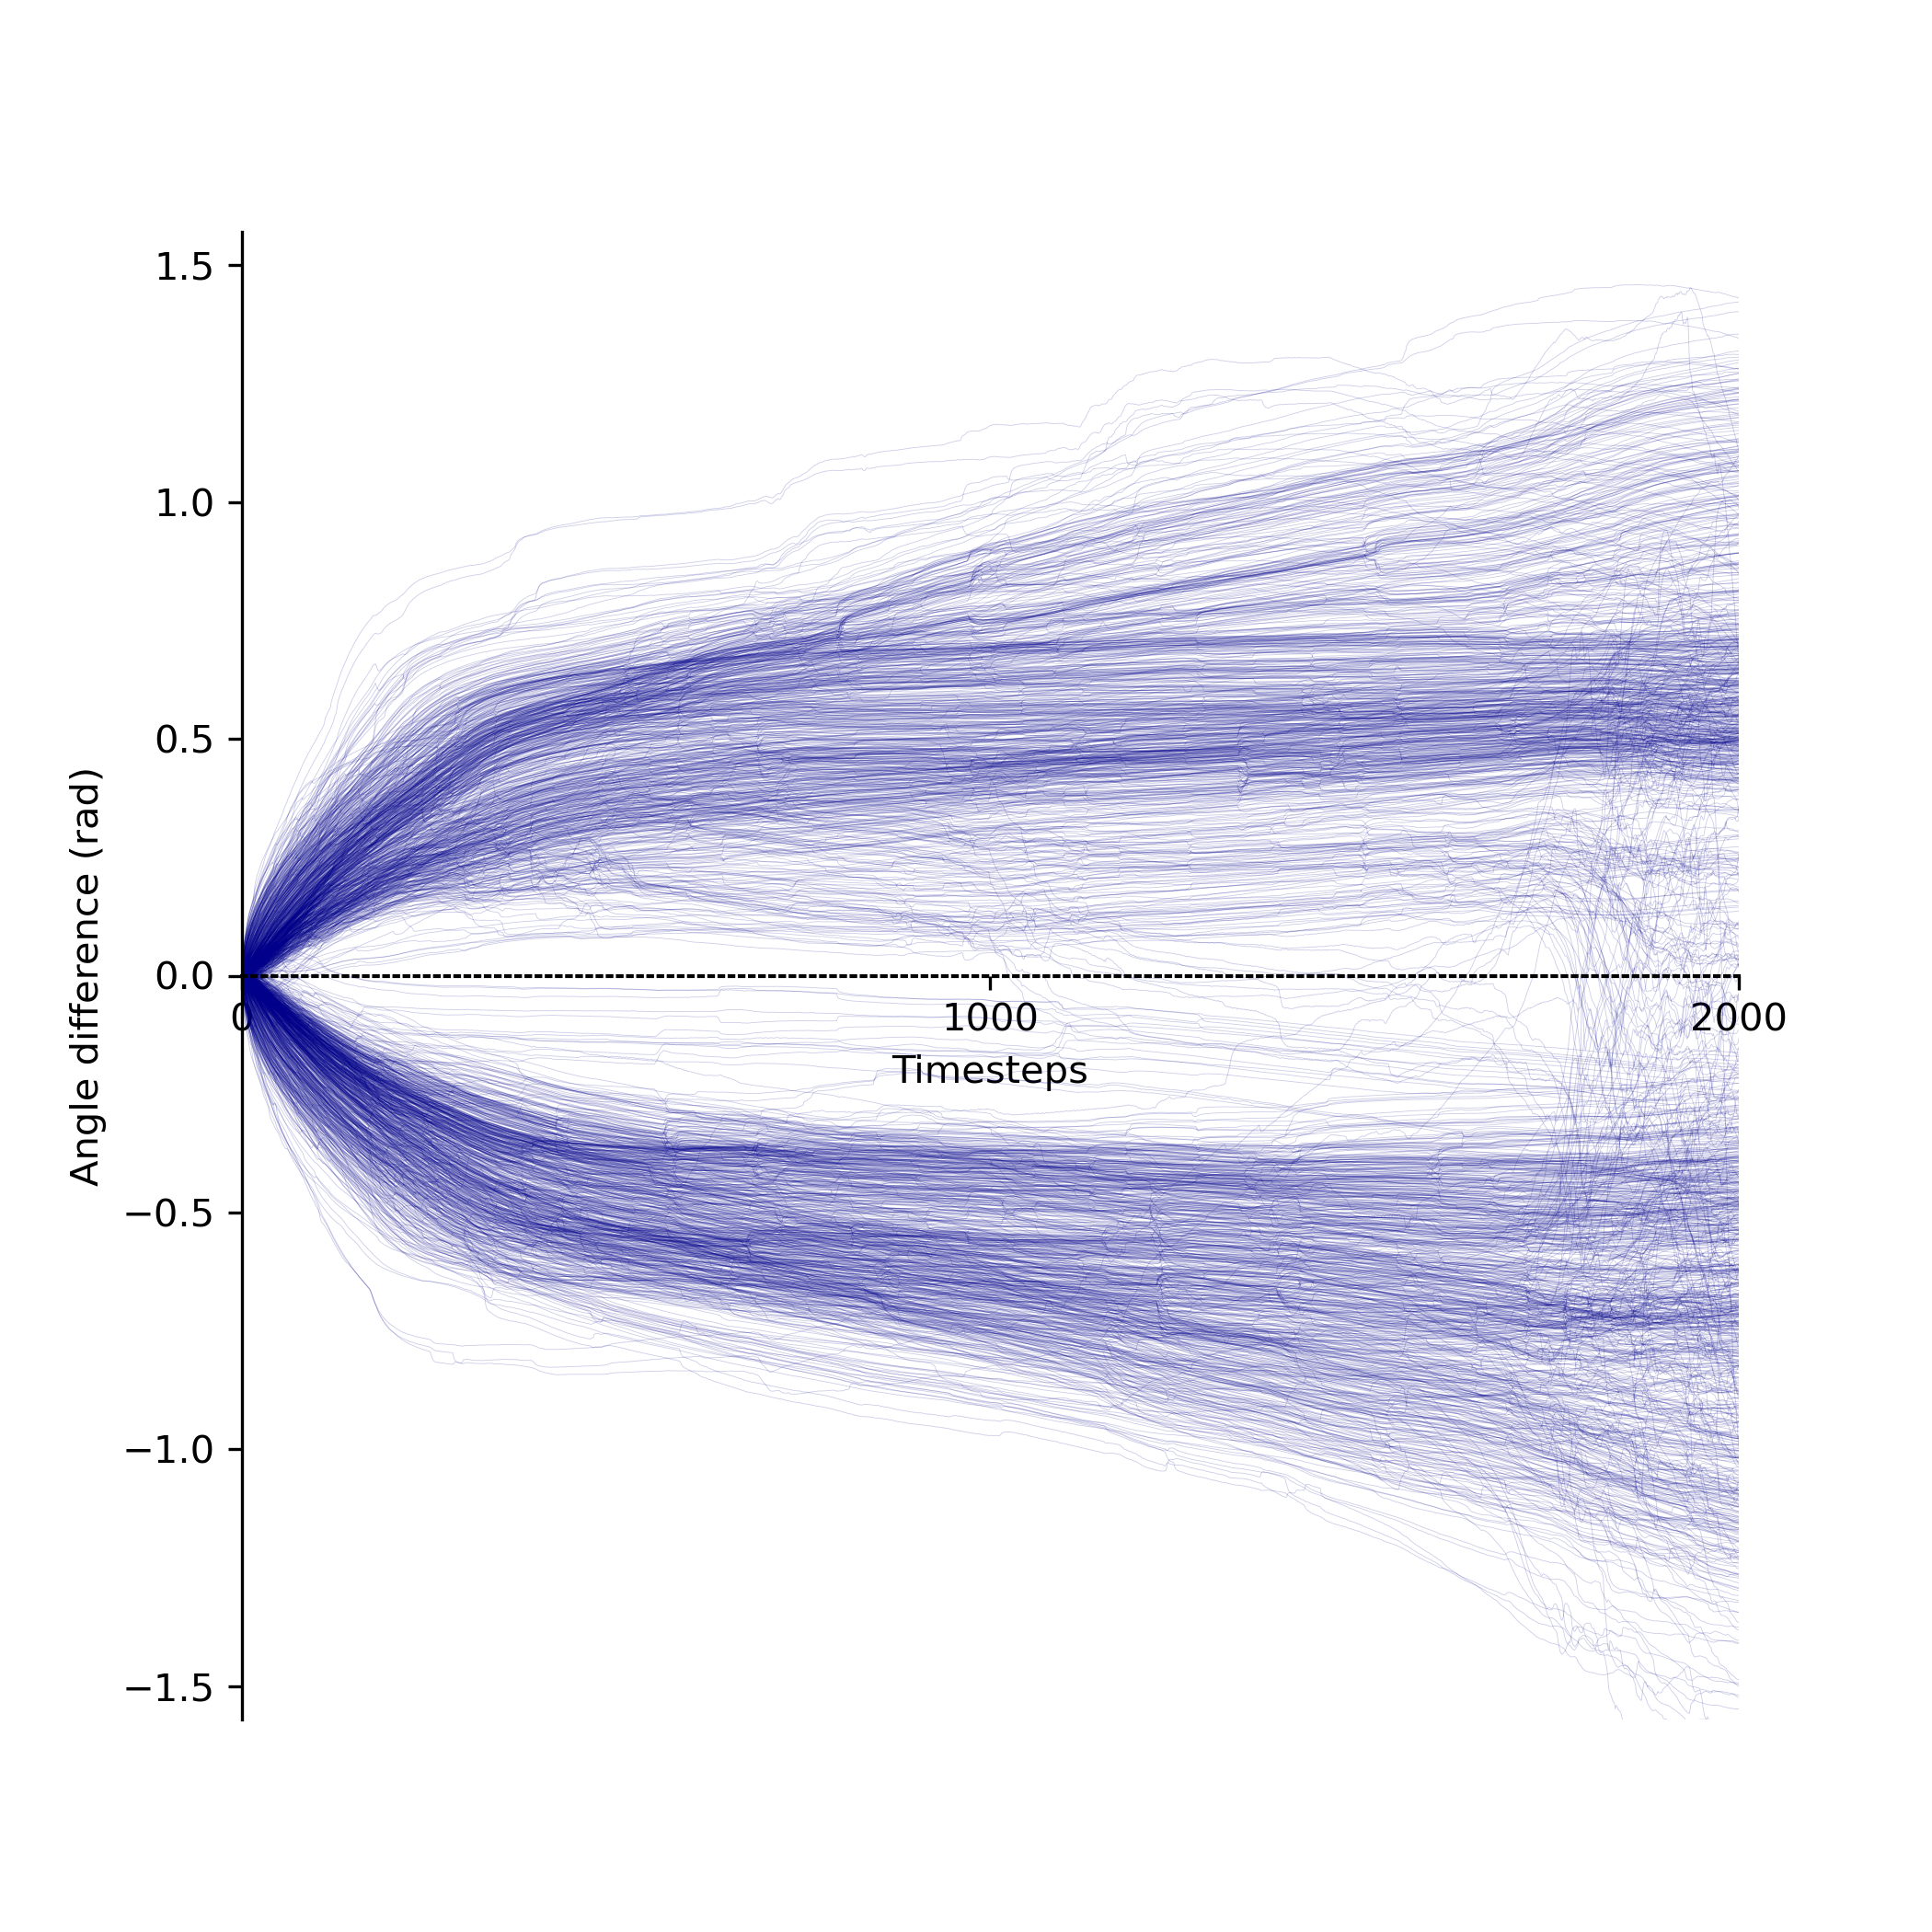
\includegraphics[width=1\linewidth]{chapters/Appendix/the_ring.png}
    \caption{Angle in cylindrical coordinates of germ band see \url{https://www.ncbi.nlm.nih.gov/pmc/articles/PMC2801059/}}
    \label{fig:enter-label}
\end{figure}
\chapter*{Code details}
\label{App:Code}
\chapter*{Sergei-analyses (tie into PCP)}
\label{App:Sergei}
\chapter*{We have not taking the following into account}
\section*{Cell shape change!}
\section*{Mitotic pressure in cephalic area}
\section*{Things that change over time}
\section*{Pressure-buckling of dorsal folds}
\section*{Pressure from yolk}
\chapter*{Other efforts we have tried in vain}

